\section{Convergence of Empirical risk minimization (ERM)}

% -----------------------------------------------------------------------------
\begin{frame}\frametitle{The learning problem}
	\begin{center} 
		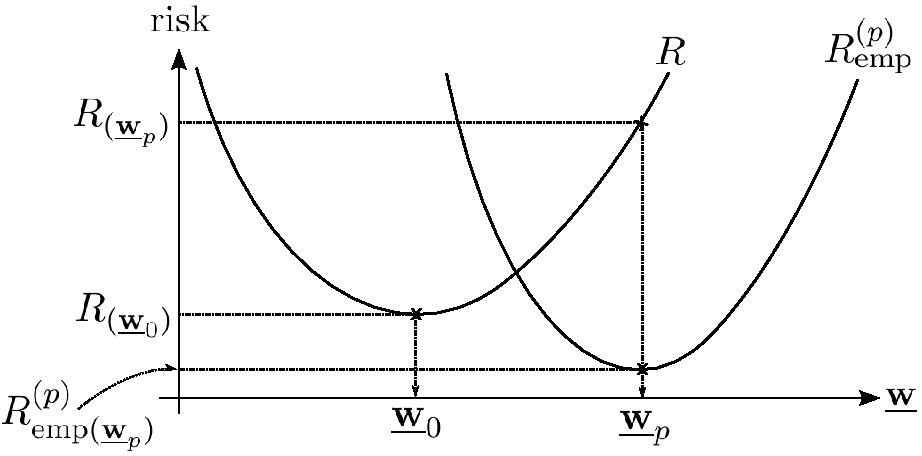
\includegraphics[height=5cm]{img/section2_fig1.pdf} 
	\end{center}
	\begin{itemize}
		\item {\footnotesize samples are drawn \iid from $P(\vec x, y_T)$\\[1mm]
			 $\quad \leadsto \quad$ $\vec w$ are random variables}
	\end{itemize}
	%{\footnotesize\hfill (see blackboard)}
\end{frame}


% -----------------------------------------------------------------------------
\definecolor{question1}{rgb}{0,0,1}
\definecolor{question2}{rgb}{0,0.5,0}
\begin{frame}\frametitle{The key questions of Statistical Learning Theory}
	\begin{center} 
		\includegraphics<1-2>[height=5cm]{img/section2_fig1_question1.pdf}
		\includegraphics<3->[height=5cm]{img/section2_fig1_question2_lessw.pdf}  
	\end{center}
	\only<1>{
		\begin{enumerate}
			\item When does inductive learning through ERM work?
				\vspace{1mm}
				\iitem{$R(\vec w_p)$ 
					should reflect the true optimal risk $R(\vec w_0)$ 
					in the limit $p \to \infty$:}
				\vspace{1mm}
				\begin{equation*}
					\lim_{p \rightarrow \infty} P \Big\{ 
							{\color{question1} \big| R_{(\vec{w}_p)}
							- R_{(\vec{w}_0)} \big| }
						\geq \eta \Big\} \;\;=\;\; 0 \,,
						\quad\text{ for all }\quad \eta > 0 \,.
				\end{equation*}
		\end{enumerate}
	} \only<2>{
		\begin{enumerate} \setcounter{enumi}{1}
			\item How strongly does $R_{(\vec{w}_p)}$ differ 
				from $R_{(\vec{w}_0)}$ for  \textbf{finite} samples?
				\vspace{1mm}
				\iitem{For a given confidence $\epsilon$, find $\eta$ such that}
				\vspace{1mm}
				\begin{equation*}
					P \Big\{ {\color{question1} 
							\big| R_{(\vec{w}_p)} - R_{(\vec{w}_0)} \big| 
						} \geq \eta \Big\} \;\;<\;\; \epsilon \,.
				\end{equation*}
		\end{enumerate}
	} \only<3>{
		\begin{enumerate} \setcounter{enumi}{2}
			\item Do training errors $R_{\text{emp}(\vec w)}$ 
				reflect generalization performance $R_{(\vec w)}$?
				\vspace{1mm}
				\iitem{\footnotesize Avoid overfitting for finite samples,
				i.e.~given confidence $\epsilon$, find $\eta$ such that: 
					%i.e.~$R_{(\vec w)} \approx R_{\mathrm{emp}(\vec w)}$:
				}
				\vspace{1mm}
				$$
					P \Big\{ {\color{question2}
							\big| R_{(\vec w)} - R_{\mathrm{emp}(\vec w)} \big|
						} > \eta \Big\} \;\;<\;\; \epsilon \,, 
						\qquad \forall \vec w \in \Lambda \,.
				$$
		\end{enumerate}
	}
\end{frame}



\begin{frame}\frametitle{\subsecname}\label{sec:convergence_erm}
			
			
			\begin{itemize}
			\item $R_{[\vec w_p]}$ is the empirical risk obtained from training the model using a finite set with $p$ points, and
			\item $R_{[\vec w_0]}$ risk obtained from training the model with inifinite many points (Don't treat the $_0$ as zero points but rather ``minimal'').
			\end{itemize}
			
			And this difference becoming smaller and smaller as we feed more points into the model. That is:
			\begin{equation}
				\lim_{p \to \infty} P\bigg\{ 
					{
						\Big|R_{[\vec w_p]} - R_{[\vec w_0]}\Big| 
					}
				\geq \eta \bigg\}\;\;=\;\; 0 \,, \quad \forall \eta > 0
				\label{eq:erm_converges_zero}
			\end{equation}
			
			Understanding what $P\bigg\{ 
					{
						\Big|R_{[\vec w_p]} - R_{[\vec w_0]}\Big| 
					}
				\geq \eta \bigg\}$ represents:
			
			\begin{itemize}
			\item We expect the model trained on $p$ points to accumulate some error $R_{[\vec w_p]}$.
			\item Training the model with a different set of $p$ points may yield a different value for $R_{[\vec w_p]}$.
			\item Training many models with $p$ will yield many values for $R_{[\vec w_p]}$.
			\item Measuring the absolute difference between every $R_{[\vec w_p]}$ we obtained and $R_{[\vec w_0]}$ will lead to ``difference values'' that follow some distribution $P\bigg\{ 
					{
						\Big|R_{[\vec w_p]} - R_{[\vec w_0]}\Big| 
					}
				\geq \eta \bigg\}$
			\item We measure the probability of the absolute difference exceeding some value $\eta$:
			\begin{equation}
			P\bigg\{ 
					{
						\Big|R_{[\vec w_p]} - R_{[\vec w_0]}\Big| 
					}
				\geq \eta \bigg\}\,, \quad \forall \eta > 0
			\end{equation}
			This is the same asking how often does traning with $p$ points yield a difference in risk above some value.
			\item Now repeat tranining these models but using a larger value for $p$.\\
			What the theory tells you is that as you increase $p$ and keeping $\eta$ fixed:
			\begin{itemize}
			\item The $R_{[\vec w_p]}$ of the models will improve and get smaller.
			\item The absolute differences $\Big|R_{[\vec w_p]} - R_{[\vec w_0]}\Big|$ will become smaller and smaller,
			\item The distribution of these differences will shift below $\eta$ (i.e. to the left of $\eta$)
			\item Less and less models will score differences $\ge \eta$
			\item Eventually, for some large $p$, the $R_{[\vec w_p]}$ of the models will be so good that the probability of finding a model that has a risk difference of $\eta$ or higher (worse performance) will vanish. And this is what \eqref{eq:risktozero} describes:
			\end{itemize}
			
			\end{itemize}
			
			\begin{equation}
				\lim_{p \to \infty} P\bigg\{ 
					{
						\Big|R_{(\vec w_p)} - R_{(\vec w_0)}\Big| 
					}
				\geq \eta \bigg\}\;\;=\;\; 0 \,, \quad \forall \eta > 0
				\label{eq:risktozero}
			\end{equation}
			
			\textbf{But} Our dataset is never going to be inifinitley large. Therefore a more realistic formulation for the convergence of ERM would be:
			
			
\end{frame}
